\graphicspath{{./chapter3/}}

\section{Chapter 3: Finite Markov Deicsion Process (MDP)}

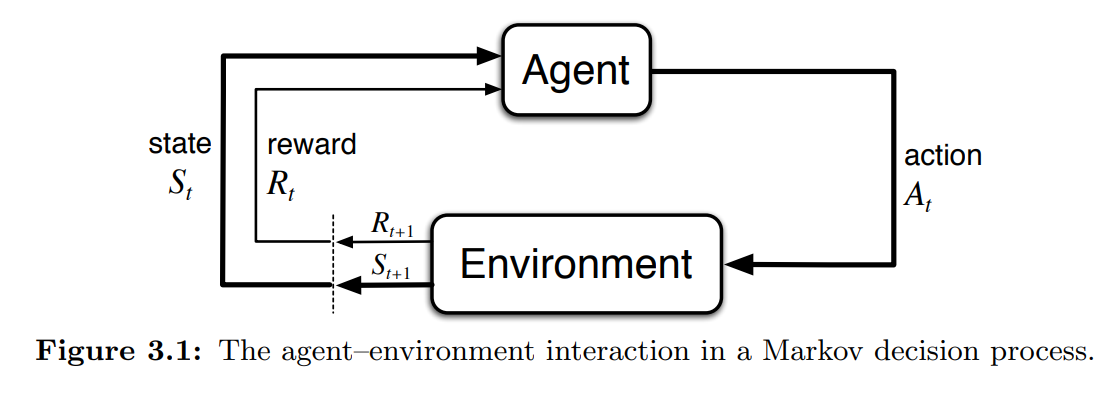
\includegraphics[scale=0.4]{./MDP.png}

\begin{itemize}
\item The reward is a consequence of an action at a state. A state (\(S_i, A_i\)) will receive a reward at time \(i+1:\ R_{i+1}\). 
\item A state or an action can be anything. A reward must be a single number. 
\item The (state, actionn, reward) triplets form the \textbf{trajectory}: 
\subitem 
\begin{equation}
    S_0, A_0, R_1, S_1, A_1, R_2, S_2, A_2, R_3,...
\end{equation}
\subitem
\begin{equation}
    p(s', r|s, a) = Pr\{S_t =s', R_t =r | S_{t-1} = s, A_{t-1} =a\},
\label{eq:four_argument_p}
\end{equation}
\subitem
\begin{equation}
    \sum_{s' \in \mathcal{S}}\sum_{r \in \mathcal{R}} p(s', r|s, a) = 1, \forall s \in S, a \in A(s).
\end{equation}

\item In general, actions can be any decision we want to learn how to make, and states can be
any interpretation of the world that might inform those actions.
\item The boundary between agent and environment is much closer to the agent than is first
intuitive. 
\item  we always consider the reward
computation to be external to the agent because it defines the task facing the agent and
thus must be beyond its ability to change arbitrarily. 
\item The general rule we follow is that anything that cannot be changed arbitrarily by
the agent is considered to be outside of it and thus part of its environment. The agent may still know everything about the environment, but still unable to solve it. E.g. solving a Rubik's cube.

\end{itemize}

\subsubsection{Exercises}

\QuestionAnswer{
 Consider the problem of driving. You could define the actions in terms of the accelerator,
steering wheel, and brake, that is, where your body meets the machine. Or you could define
them farther out—say, where the rubber meets the road, considering your actions to be tire
torques. Or you could define them farther in—say, where your brain meets your body, the
actions being muscle twitches to control your limbs. Or you could go to a really high level and
say that your actions are your choices of where to drive. What is the right level, the right place
to draw the line between agent and environment? On what basis is one location of the line
to be preferred over another? Is there any fundamental reason for preferring one location over
another, or is it a free choice?
}
{
There's a trade-off between state-action space complexity, computational expense and accuracy.
If we draw the boundary at the brain we would create a state-action space contingent on the
number of neurons in the brain and their interplay with physical actions like turning the steering
wheel; too large to be stored or computed efficiently. Equally, if we draw the boundary at the
journey level, then we miss the detail required to act on second-by-second state changes on the
road that could lead to a crash. The fundamental limiting factor in this selection is whether the
goal can be achieved safely at your chosen layer of abstraction, indeed this feels like one of the
tasks of engineering more widely
}





% -------------------------------------------- SUBSECTION --------------------------------------------
\subsection{Goals and Rewards}

\begin{itemize}
    \item The \textit{reward hypothesis}: "That all of what we mean by goals and purposes can be well thought of as
    the maximization of the expected value of the cumulative sum of a received
    scalar signal (called reward)."
    \item It is thus critical that the rewards we set up truly indicate what we want accomplished.
    In particular, the reward signal is not the place to impart to the agent prior knowledge
    about \textit{how} to achieve what we want it to do. For example, a chess-playing agent should
    be rewarded only for actually winning, not for achieving subgoals such as taking its
    opponent's pieces or aining control of the center of the board. If achieving these sorts
    of subgoals were rewarded, then the agent might find a way to achieve them without
    achieving the real goal. For example, it might find a way to take the opponent's pieces
    even at the cost of losing the game. 
    \item The reward signal is your way of communicating to
    the agent \textit{what} you want achieved, not \textit{how} you want it achieved.
\end{itemize}






% --------------------------------------------- SUBSECTION --------------------------------------------
\subsection{Returns and Episodes}

\begin{itemize}
\item An agent needs to maximize the cummulative reward in the long run, not just the immediate reward. 
\item Can we use the sum of all rewards as the metric? it can grow without bound if the task doesn't have a terminal state.
\item Instead, use discounts: 
\subitem 
\begin{align}
    G_t \doteq R_{t+1} + \gamma R_{t+2} + \gamma^2 R_{t+3} + \dotsb &= \sum_{k=0}^{\infty} \gamma^k R_{t+k+1} \\     \label{eq:G_definition}
    G_t \doteq R_{t+1} + \gamma R_{t+2} + \gamma^2 R_{t+3} + \dotsb &= R_{t+1} + \gamma (R_{t+2} + \gamma R_{t+3} + \dotsb) = R_{t+1} + \gamma G_{t+1} 
\end{align}
\end{itemize}

\subsubsection{Exercises}

\QuestionAnswer{
Suppose you treated pole-balancing as an episodic task but also used
discounting, with all rewards zero except for 1 upon failure. What then would the
return be at each time? How does this return differ from that in the discounted, continuing
formulation of this task?

}
{
For \textit{episodic} tasks, each episode has a terminate state. And the corresponding metric, with discounts, for each episode is:
\begin{equation*}
    G_t \doteq R_{t+1} + \gamma R_{t+2} + \dotsb + \gamma^{T-t-1} R_T = 0 + \gamma^{T-t-1} R_T = \gamma^{T-t-1} (-1) = -\gamma^{T-t-1}.
\end{equation*}
}

\QuestionAnswer{
Imagine that you are designing a robot to run a maze. You decide to give it a
reward of +1 for escaping from the maze and a reward of zero at all other times. The task
seems to break down naturally into episodes—the successive runs through the maze—so
you decide to treat it as an episodic task, where the goal is to maximize expected total
reward (3.7). After running the learning agent for a while, you find that it is showing
no improvement in escaping from the maze. What is going wrong? Have you effectively
communicated to the agent what you want it to achieve?
}
{
    We only reward it for exiting the maze, but did not penalize it for the time it takes to exit the maze. 
We can improve on this by giving negative rewards as the time it takes to exit the maze increases.

}


\QuestionAnswer{
    Suppose  \(\gamma = 0.5\) and the following sequence of rewards is received \(R_1 = 1,
R_2 = 2, R_3 = 6, R_4 = 3, \text{ and } R_5 = 2, \text{ with } T = 5\). What are \(G_0, G_1, ..., G_5\)? Hint:
Work backwards.
}
{
We know \(G_t = R_{t+1} + \gamma \cdot G_{t+1}\). So 
\begin{enumerate}
    \item \(G_5 = 0\)
    \item \(G_4 = R_5 + \gamma \cdot G_5 = 2 + 0 = 2\)
    \item \(G_3 = R_4 + \gamma \cdot G_4 = 3 + 0.5 \cdot 2 = 4\)
    \item \(G_2 = R_3 + \gamma \cdot G_3 = 6 + 0.5 \cdot 4 = 8\)
    \item \(G_1 = R_2 + \gamma \cdot G_2 = 2 + 0.5 \cdot 8 = 6\)
    \item \(G_0 = R_1 + \gamma \cdot G_1 = 1 + 0.5 \cdot 6 = 4\)
\end{enumerate}
}






% --------------------------------------------- SUBSECTION --------------------------------------------
\subsection{Unified Formulation for Episodic and Continuing Tasks}

\begin{itemize}
    \item Use a self-absorbing state \(S_T\) that returns a reward of 0 to represent the termination of an episode.
    \subitem 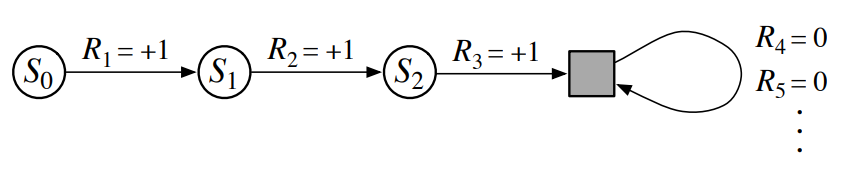
\includegraphics[scale=0.3]{./self_absorb.png}
    \item The sum remains the same for both terminating (episodic) and continuing task. 
    \item To include discounting, either \(\gamma = 1\) or \(T = \infty\) but not both. Cause if both are true, then the sum diverges.
\end{itemize} 










% --------------------------------------------- SUBSECTION --------------------------------------------
\subsection{Value Functions and Action-Value Functions}

\begin{itemize}
    \item The \textbf{state-value function} for a policy $\pi$, denoted $v_{\pi}(s)$, is the expected return when starting in state $s$ and following policy $\pi$ thereafter. It is formally defined as:
    \begin{equation}
    v_{\pi}(s) \doteq \mathbb{E}_{\pi}[G_t | S_t=s] = \mathbb{E}_{\pi}\left[\sum_{k=0}^{\infty} \gamma^k R_{t+k+1} \middle| S_t=s\right], \quad \text{for all } s \in \mathcal{S}
    \end{equation}
    where $\mathbb{E}_{\pi}[\cdot]$ denotes the expected value given that the agent follows policy $\pi$, $G_t$ is the total discounted return from time step $t$, $S_t$ is the state at time $t$, $R_{t+k+1}$ is the reward at time step $t+k+1$, and $\gamma$ is the discount factor. The value of the terminal state, if any, is always zero.

    \item Similarly, the \textbf{action-value function} for a policy $\pi$, denoted $q_{\pi}(s, a)$, is the expected return starting from state $s$, taking action $a$, and thereafter following policy $\pi$. It is formally defined as:
    \begin{equation}
        q_{\pi}(s, a) \doteq \mathbb{E}_{\pi}[G_t | S_t=s, A_t=a] = \mathbb{E}_{\pi}\left[\sum_{k=0}^{\infty} \gamma^k R_{t+k+1} \middle| S_t=s, A_t=a\right]
    \end{equation}
    where $A_t$ is the action taken at time step $t$.

    \item  $v_{\pi}$ measures \textit{how good} a \textit{state} is, while $q_{\pi}$ measures \textit{how good} a \textit{state-action pair} is.

    \item The \textbf{Bellman equation}  states that the value of the start state must equal the (discounted) value of the expected next state, plus the \textit{expected} reward along the way:
    \begin{align} % Use align (not align*) to enable numbering
        v_{\pi}(s) & \doteq \mathbb{E}_{\pi}[G_t | S_t=s] \nonumber \\ % Add \nonumber to suppress the number for this line
        & = \mathbb{E}_{\pi}[R_{t+1} + \gamma G_{t+1} | S_t=s] \nonumber \\ % Add \nonumber here too
        & = \sum_a \pi(a|s) \sum_{s'} \sum_r p(s', r | s, a) \left[r + \gamma \mathbb{E}_{\pi}[G_{t+1} | S_{t+1}=s']\right] \nonumber \\ % And here
        & = \sum_a \pi(a|s) \sum_{s',r} p(s', r | s, a) \left[r + \gamma v_{\pi}(s')\right], \quad \text{for all } s \in \mathcal{S}, \label{eq:bellman_value} % This line will be numbered automatically
    \end{align}
    
    \item $v_{\pi}$ satisfies a recursive relationship and is a unique solutionn to Bellman's equation.\\item $v_{\pi}$ satisfies a recursive relationship and is a unique solutionn to Bellman's equation.\
    \item Similarly, the Bellman equation for the action-value function $q_{\pi}(s, a)$ is:
    \begin{align}
        q_{\pi}(s, a) & \doteq \mathbb{E}_{\pi}[G_t | S_t=s, A_t=a]  \nonumber \\
        & = \mathbb{E}_{\pi}[R_{t+1} + \gamma G_{t+1} | S_t=s, A_t = a] \nonumber \\ 
        & = \sum_{s'} \sum_r p(s', r | s, a) \left[r + \sum_{a'} \pi(a' | s') \gamma \mathbb{E}_{\pi}[G_{t+1} | S_{t+1}=s', A_{t+1}=a']\right] \nonumber \\ 
        & = \sum_{s'} \sum_r p(s', r | s, a)  \left[r + \gamma \sum_{a'} \pi(a' | s') q_{\pi}(s', a')\right] \nonumber \\
        & = \sum_{s', r} p(s', r | s, a)\left[r +  \gamma \sum_{a'} \pi(a' | s') q_{\pi}(s', a')\right] \label{eq:bellman_action}
    \end{align}
\end{itemize}



\subsubsection{Exercises}

\QuestionAnswer{ % Question
 If the current state is $S_t$, and actions are selected according to a stochastic
policy $\pi$, then what is the expectation of $R_t+1$ in terms of $\pi$ and the four-argument
function $p$ in (\ref{eq:four_argument_p})?
}
{ % Answer
\begin{equation*}
    \mathbb{E}_{\pi}[R_{t+1} | S_t] = \sum_{a} \pi(a | S_t) \sum_{s' \in \mathcal{S}} \sum_{r \in \mathcal{R}} r \cdot p(s', r | S_t, A_t = a).
\end{equation*}
}


\QuestionAnswer{
 Give an equation for \(v_\pi\) in terms of \(q_\pi\) and \(\pi\).
}
{
We have \(v_\pi(s) = \mathbb{E}_{\pi}[G_t | S_t = s] = \sum_{a} \pi(a | s) q_\pi(s, a)\). This is the expected value of \(q_\pi\) over all actions \(a\) taken in state \(s\) according to policy \(\pi\).

\begin{gather*} 
    v_\pi(s) = \sum_{a} \pi(a | s)\ \mathbb{E}_{\pi}[G_t\ |\ S_t = s, A_t = a]. \\ % Use \\ for a new line
    q_\pi(s, a) = \mathbb{E}_{\pi}[G_t\ |\ S_t = s, A_t = a]. \\ % Use \\ for a new line
    \Rightarrow v_\pi(s) = \sum_{a} \pi(a | s)\ q_\pi(s, a). % No \\ on the last line
\end{gather*}
}


Figure 3.2 (left) shows a rectangular gridworld representation
of a simple finite MDP. The cells of the grid correspond to the states of the environment. At
each cell, four actions are possible: north, south, east, and west, which deterministically
cause the agent to move one cell in the respective direction on the grid. Actions that
would take the agent off the grid leave its location unchanged, but also result in a reward
of 1. Other actions result in a reward of 0, except those that move the agent out of the
special states $A$ and $B$. From state $A$, all four actions yield a reward of +10 and take the
agent to $A'$
From state $B$, all actions yield a reward of +5 and take the agent to $B'$

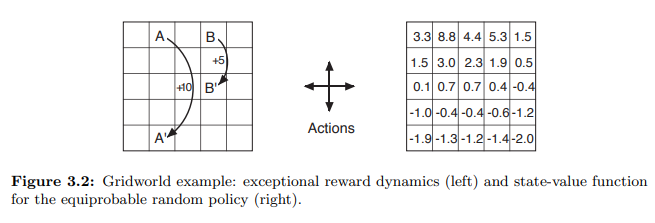
\includegraphics[scale=0.7]{./gridworld.png}

\QuestionAnswer{
    The Bellman equation (\ref{eq:bellman_value}) must hold for each state for the value function
    $v_\phi$ shown in Figure 3.2 (right) of the gridworld above. Show numerically that this equation holds
    for the center state, valued at +0.7, with respect to its four neighboring states, valued at
    +2.3, +0.4, 0.4, and +0.7. (These numbers are accurate only to one decimal place.) 
}
{
    Using the Bellman equation, we have:
    \begin{align*}
        v_\pi(s) & = \sum_a \pi(a|s) \sum_{s',r} p(s', r | s, a) \left[r + \gamma v_\pi(s')\right] \\
        & = 0.25 \cdot (0.9 \times 0.7) + 0.25 \cdot (0.9 \times 2.3) + 0.25 \cdot (0.9 \times 0.4) + 0.25 \cdot (0.9 \times -0.4) \\
        & = 0.25 \cdot 0.9 \cdot (0.7 + 2.3 + 0.4 - 0.4) \\
        & = 0.675 \approx 0.7.
    \end{align*}
}

\QuestionAnswer{
    In the gridworld example, rewards are positive for goals, negative for
running into the edge of the world, and zero the rest of the time. Are the signs of these
rewards important, or only the intervals between them? Prove, using (\ref{eq:G_definition}), that adding a
constant $c$ to all the rewards adds a constant, $v_c$, to the values of all states, and thus
does not affect the relative values of any states under any policies. What is $v_c$ in terms
of $c$ and $\gamma$?
} 
{
    Adding a constant \(c\) to all rewards results in the following equation:
    \begin{align*}
        G_t & = \sum_{k=0}^{\infty} \gamma^k (R_{t+k+1} + c) \\
        & = \sum_{k=0}^{\infty} \gamma^k R_{t+k+1} + \sum_{k=0}^{\infty} \gamma^k c \\
    \end{align*}
    Thus, the value of each state increases by:
    \begin{align*}
        v_c & = \sum_{k=0}^{\infty} \gamma^k c \\
        & = c \cdot \sum_{k=0}^{\infty} \gamma^k \\
        & = c \cdot \frac{1}{1 - \gamma} \quad (\text{for } |\gamma| < 1)\\
        & = \frac{c}{1 - \gamma}.
    \end{align*}
}


\QuestionAnswer{
    Now consider adding a constant c to all the rewards in an episodic task,
    such as maze running. Would this have any effect, or would it leave the task unchanged
    as in the continuing task above? Why or why not? Give an example. 
}{
Yes, it would affect the agent. Episodes have a finite length, so the total return is finite. 
Adding a constant \(c\) to all rewards would change the total return for each episode by \(c\) times the number of time steps in that episode.
This would affect the agent's learning and policy, as it would now be incentivized to complete episodes faster or slower depending on the sign of \(c\). 
For example, if \(c\) is positive, it will overwhelm the negative rewards for "bad decisions", so the agent is not incentivized to learn from its mistakes, and continues 
collecting intermediate rewards indefinitely.

\textit{Consequently, adding a constant to all rewards in an episodic task can alter the \textbf{relative} values of different states and policies, 
and may therefore change the optimal policy, especially by influencing the agent's preference for \textbf{episode length}.}

Consider a simple maze with a starting state S and a terminal goal state T.
The agent receives a reward $R_{step}$ for each step taken. The episode ends upon reaching T.
\begin{itemize}
    \item Path 1 (Short, 2 steps toTG):
    Total Return $G_1 = \sum_{k=1}^{2} R_{step} = 2 \times (-1) = -2$.
    \item Path 2 (Long, 3 steps to G):
    Total Return $G_2 = \sum_{k=1}^{3} R_{step} = 3 \times (-1) = -3$.
\end{itemize}
Since $-2 > -3$, Path 1 is preferred.

Now, add a constant $c = +5$ to all rewards. The new reward per step is $R'_{step} = R_{step} + c = -1 + 5 = 4$.
The new total return $G'_t$ for an episode of length $L$ starting from a state leading to original return $G_t$ is $G'_t = G_t + L \cdot c$.

\begin{itemize}
    \item Path 1 (Short, $L=2$ steps):
    $G'_1 = G_1 + 2c = -2 + 2(5) = -2 + 10 = 8$.
    Alternatively, $G'_1 = 2 \times R'_{step} = 2 \times 4 = 8$.
    \item Path 2 (Long, $L=3$ steps):
    $G'_2 = G_2 + 3c = -3 + 3(5) = -3 + 15 = 12$.
    Alternatively, $G'_2 = 3 \times R'_{step} = 3 \times 4 = 12$.
\end{itemize}
Since $12 > 8$, Path 2 (the longer path) is now preferred. The addition of a positive constant favored the policy leading to a longer episode.

}

\QuestionAnswer{
    What is the Bellman equation for action values, that
is, for $q_\pi$? It must give the action value $q_\pi(s, a)$ in terms of the action
values, $q_\pi(s', a')$, of possible successors to the state-action pair $(s, a)$.
Hint: The backup diagram to the right corresponds to this equation.
Show the sequence of equations analogous to (\ref{eq:bellman_action}), but for action
values.
} 
{
    See (\ref{eq:bellman_action}). 
}